\section{Notion of identity.} \label{identity}

The identity matrix $I$ is the one that satisfies that $AI = IA = A$. It's interesting to look for a similar notion in cubrices, however, we soon discover our expectations to be challenged.

\subsection{I's uniqueness.} \label{identity-unique}

Let $A, I \in M_{n} (\mathbb{K})$ such that $IIA = A$ (the reasoning works regardless of the product's order). We start from three assumptions:

\begin{itemize}
	\item No element from $A$ is zero.
	\item Elements from $I$ don't depend on ones from $A$.
	\item The identity cubrix $I$ is unique.
\end{itemize}

By definition:

$$A_{ijk} = (I \cdot I \cdot A)_{ijk} = \sum\limits_{l=1}^{n} I_{ilk} \cdot I_{ljk} \cdot A_{ijl}$$

Because we supposed that $I$ is independent from $A$, this expression can only yield $A_{ijk}$ from the sum's term $A_{ijl}$. In other words, $I_{ilk} I_{ljk} = \delta_{lk}$, where $\delta_{lk}$ is the \textit{Kronecker delta}, an expression we'll frequently use and which is equivalent to:

\begin{equation}
	\delta_{ab} =
	\begin{cases}
		1 & \text{if } a = b \\
		0 & \text{if } a \neq b
	\end{cases}
\end{equation}

According to the previous expressions we can derive a formula for $I_{ijk}$ by subtle manipulation of subindices. See $I_{ilk}$ and note that saying that it is equal to $1$ if $l$ takes $k$'s value is equivalent to saying that it is equal to $1$ if its $j$ is equal to its $k$. In other words, $I_{ijk} = \delta_{jk}$. But applying the same reasoning over $I_{ljk}$ we get that $I_{ijk} = \delta_{ik}$. The only way to avoid this contradiction is to establish that $I_{ijk} = \delta_{jk} \delta_{ik}$, but this necessarily leaves out multiple elements of $A$. (See Appendix \ref{appendix-1} for a complete elaboration on the $M_2 (\mathbb{K})$ particular case if help is needed to clarify the pattern).

At least one of our assumptions must be wrong, and it would be optimal for it to be the third one (on the identity's uniqueness).

\subsection{Identity as a pair.} \label{identity-pair}

We say that $I, J \in M_{n} (\mathbb{K})$ form an \textit{identity pair} if they satisfy that $AIJ = A$ (we'll later explore the influence of the order of factors). Once again, using the product's definition:

$$A_{ijk} = (AIJ)_{ijk} = \sum\limits_{l=1}^{n} A_{ilk} I_{ljk} J_{ijl}$$

This time, the conditions to be satisfied are:

\begin{itemize}
	\item $I_{ljk} = J_{ijl}^{-1}$ if $l = j$ and $I_{ljk} J_{ijl} = 0$ if $l \neq j$.
	\item $J_{ijl} = I_{ljk}^{-1}$ if $l = k$ and $J_{ijl} I_{ljk} = 0$ if $l \neq k$.
\end{itemize}

Any two cubrices that fulfill these conditions will be considered an \textit{identity pair}, and they will satisfy that $AIJ = A$. It's obvious that if $\mathbb{K}$ is a field, there will be infinitely many identity pairs, whereas if it's a commutative unitary ring, only the following ones will exist.

\subsection{The three Kroneckers.} \label{identity-kronecker}

For simplicity and standardization we can set all terms which must be the inverse of others to be equal to $1$, whereas we set all terms which must cancel out to be equal to $0$.

That is to say, for $(AIJ)_{ijk} = A_{ijk}$, then $I_{ljk} = J_{ijl} = \delta_{jl}$. With a reasoning very similar to the one in section \ref{identity-unique}, we can make these expressions independent from the $l$ subindex:

$$I_{ijk} = \delta_{ij}$$

Having in mind that the identity pair isn't commutative, it's easy to do something similar both for $I_2 A J_2$ and $I_3 J_3 A$ (commuting $I$ and $J$ won't produce new cubrices, but only commute their names). With $\Delta_{ab} = (\delta_{ab})$, we get that:

$$A = A \Delta_{ij} \Delta_{jk} = \Delta_{ij} A \Delta_{ik} = \Delta_{jk} \Delta_{ik} A$$

\newpage

With this we conclude that there exist three standard identity pairs grounded on the three Kroneckers. It isn't immediately obvious which pattern to take out from this result. In any case, it's intriguing to observe the cubrices drawn by each Kronecker. Let's take their complete three-dimensional representations.

\begin{figure}[H]
	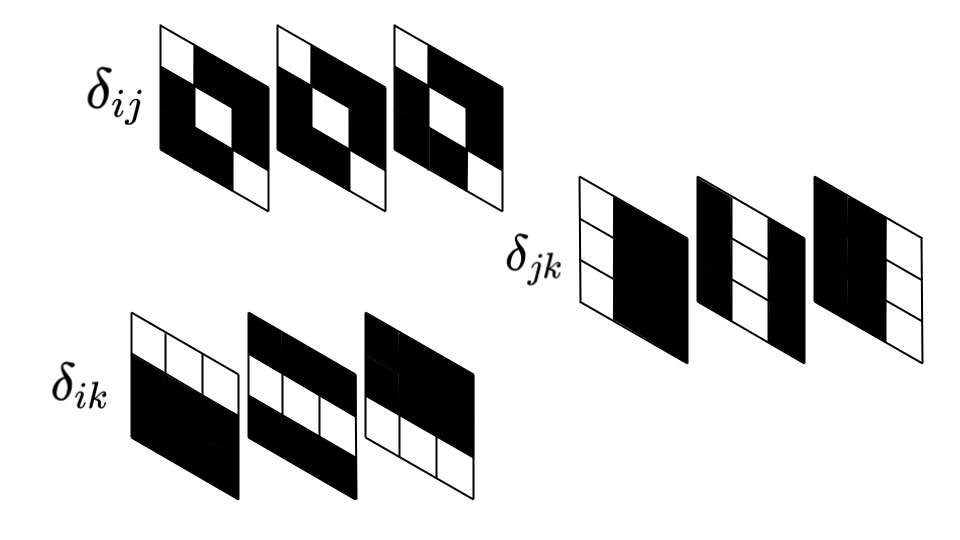
\includegraphics[width=\linewidth]{media/kroneckers.png}
	\caption{Complete three-dimensional representation of $\Delta_{ij}$, $\Delta{jk}$ y $\Delta{ik}$ (cells equal to $1$ in white and those equal to $0$ in black).}
\end{figure}

It can be useful to group and rename terms in the following way. If $I_{ijk} = 1$, then:

\begin{itemize}
	\item $A = A \Delta_{ij} I = A I \Delta_{jk}$.
	\item $A = \Delta_{ij} A I = I A \Delta_{ik}$.
	\item $A = \Delta_{jk} I A = I \Delta_{ik} A$.
\end{itemize}

\newpage
